\documentclass{article}
\usepackage{graphicx}
\usepackage[utf8]{inputenc}
\usepackage{amsmath, amssymb, latexsym}

\usepackage{pgfplots}
\usepackage{algorithm}
\usepackage[noend]{algpseudocode}
\usepackage{tikz}
\usepackage{nicefrac}
\pgfplotsset{every axis legend/.append style={
at={(0,0)},
anchor=north east}}
\usetikzlibrary{shapes,positioning,intersections,quotes}
\usetikzlibrary{arrows.meta,
                bending,
                intersections,
                quotes,
                shapes.geometric}
                
\definecolor{darkgreen}{rgb}{0.0, 0.6, 0.0}
\definecolor{darkred}{rgb}{0.7, 0.0, 0.0}
\makeatletter
\def\BState{\State\hskip-\ALG@thistlm}
\makeatother
\title{Week 3}
\begin{document}
\pagenumbering{gobble}
\maketitle
\newpage
\pagenumbering{arabic}

\section*{Matrices - overview}
\begin{itemize}
  \item Rectangular array of numbers written between square brackets.
  \item 2D array.
  \item Named as capital letters (A,B,X,Y).
  \item It allows you to organize, index, and access a large amount of data.
  \item Dimension of a matrix are [Rows x Columns].
  \item $A_{(i,j)} =$ entry in $i^{th}$ row and $j^{th}$ column.
\end{itemize}

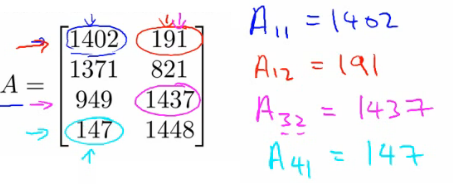
\includegraphics[width=0.8\textwidth]{resources/matrix_element}

\section*{Vectors - overview}
\begin{itemize}
  \item n by 1 matrix.
  \item Usually referred to as a lower case letter
  \item $v_i $ is an $i^{th}$ element.
  \item It allows you to organize, index, and access a large amount of data.
  \item Dimension of a matrix are [Rows x Columns].
  \item $A_{(i,j)} =$ entry in $i^{th}$ row and $j^{th}$ column.
\end{itemize}

\begin{align*}
  y & = \begin{bmatrix}
    x_{1}  \\
    x_{2}  \\
    \vdots \\
    x_{m}
  \end{bmatrix}
\end{align*}

\section*{Matrix manipulation}

\subsection*{Addition}

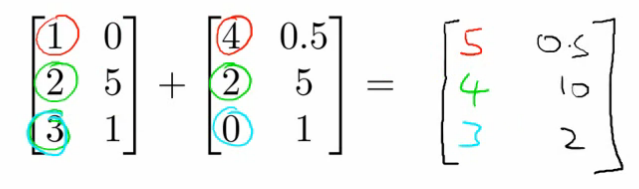
\includegraphics[width=0.8\textwidth]{resources/matrix_addition}

\subsection*{Multiplication by scalar}

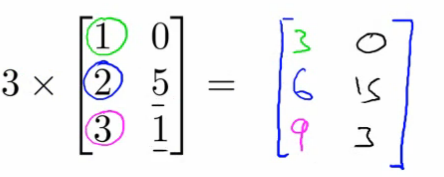
\includegraphics[width=0.7\textwidth]{resources/matrix_mult_scalar}

\subsection*{Multiplication by vector}

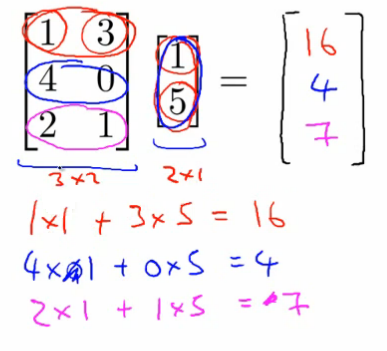
\includegraphics[width=0.7\textwidth]{resources/matrix_mult_vector}

\subsection*{Multiplication by matrix}

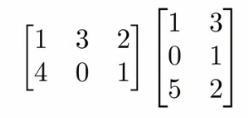
\includegraphics[width=0.5\textwidth]{resources/matrix_mult_matrix}

\begin{itemize}
  \item Take matrix A and multiply by the first column vector from B.
  \item Take the matrix A and multiply by the second column vector from B.
\end{itemize}

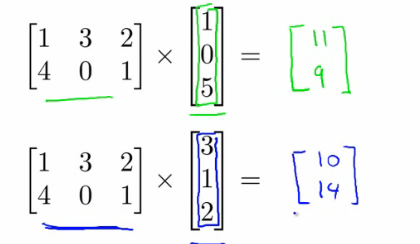
\includegraphics[width=0.8\textwidth]{resources/matrix_mult_column}

\subsection*{Implementation/use}

\begin{itemize}
  \item House prices. However, we now have three hypotheses and the same data set.
  \item We can use matrix-matrix multiplication to efficiently apply all three hypotheses to all data.
  \item For example, suppose we have four houses and we wish to guess their prices. There are three opposing hypotheses. Because our hypothesis is only one variable, we convert our data (home sizes) vector into a 4x2 matrix by adding an extra column of 1s.
\end{itemize}

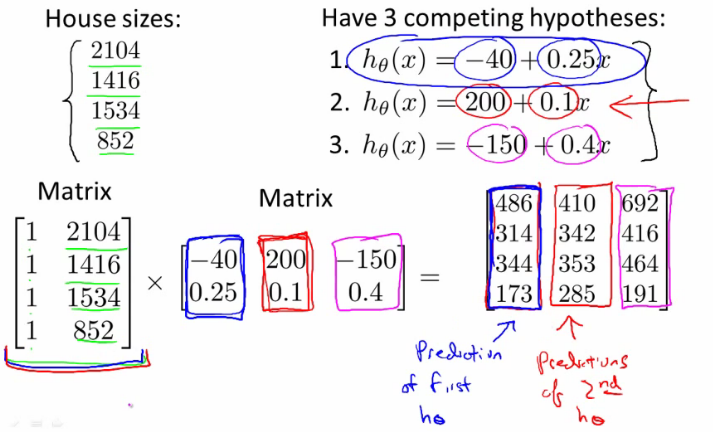
\includegraphics[width=\textwidth]{resources/matrix_mult_use}

~\\
\section*{Matrix multiplication properties}

\subsection*{Lack of Commutativity}

When working with raw numbers/scalars multiplication is commutative:

$$3 \cdot 5 == 5 \cdot 3$$

~\\
This is not always true for matrix:

$$A \times B \neq B \times A$$

\subsection*{Associativity}

When working with raw numbers/scalars multiplication is associative:

$$3 \cdot 5 \cdot 2 == 3 \cdot 10 == 15 \cdot 2$$

~\\
This also holds true for matrix:

$$A \times (B \times C) ==  (A  \times B) \times C$$

\subsection*{Identity matrix}

When working with raw numbers/scalars 1 is always the identity element:

$$z \cdot 1 = z$$

~\\
In matrices we have an identity matrix called I:

\begin{equation*}
  I =
  \begin{pmatrix}
    1 & 0 & 0 \\
    0 & 1 & 0 \\
    0 & 0 & 1
  \end{pmatrix}
\end{equation*}

~\\
If multiplication between matrices A and I is possible:

$$A \times I = A$$

\section*{Matrix inverse}

When working with raw numbers/scalars multiplication we can usually take their inverse:

$$ x \cdot \frac{1}{x} = 1$$

~\\
In the space of real numbers not everything has an inverse. E.g. 0 does not have an inverse!

~\\
The only matrices that have an inverse are square matrices.\\

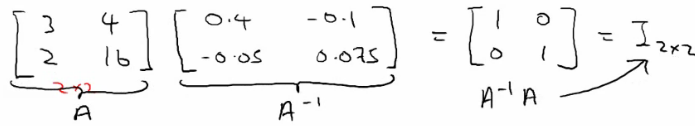
\includegraphics[width=\textwidth]{resources/matrix_inverse}

~\\
There are numerical methods used for finding the inverses of matrices.

\section*{Matrix transpose}

If A is an $m \times n$ matrix B is a transpose of A.
Then B is an $n \times m$ matrix $A_{(i,j)} = B_{(j,i)}$.

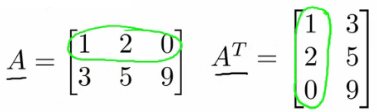
\includegraphics[width=0.5\textwidth]{resources/matrix_transpose}


\end{document}